\documentclass[11pt,xcolor={dvipsnames},hyperref={pdftex,pdfpagemode=UseNone,hidelinks,pdfdisplaydoctitle=true},usepdftitle=false]{beamer}

\usepackage{microtype}
\usepackage[slovak]{babel}
\usepackage[utf8]{inputenc}
\usepackage[T1]{fontenc}

\usepackage{csquotes}
\usepackage{multicol}
\usepackage[export]{adjustbox}
\usepackage{svg}

\usetheme[
nogauge,
nologo,
nomail,
%amurmapleblue
]{Amurmaple}


\title[SPAR]{SPAR - Systém na podporu analýzy rizík}
\author[A.~Kica]{Bc. Anton Kica}
%\subtitle{documentation\quad v.1.3}
\institute[FMFI]{FMFI\\Univerzita Komenského v Bratislave}
\date{Máj 14, 2025}
%\titlegraphic{\includegraphics[width=4cm]{logo.png}}
%\mail{chupin@ceremade.dauphine.fr}
%\webpage{www.ceremade.dauphine.fr/~chupin/}
\collaboration{školiteľ: doc. RNDr. Daniel Olejár, PhD}

%\bibliography{biblio.bib}
\usefonttheme{serif}

\begin{document}

\maketitle
\sepframe[title={Obsah}]

\section{úvod do problematiky}
\begin{frame}
  \frametitle{úvod do problematiky}
\end{frame}

\begin{frame}
  \frametitle{čo to je analýza rizík?}
  zúžené na oblasť informačnej bezpečnosti, analýza rizík:
  \begin{itemize}
    \item je proces identifikácie relevantných hrozieb informačných aktív a odhadnutia súvisiaceho výsledného rizika
    \item jej cieľom je znížiť úroveň rizika na akceptovateľnú úroveň pomocou vhodných protiopatrení
    \item umožňuje systematickú kontrolu celkového rizika
    \item je súčasťou systému riadenia informačnej bezpečnosti (ISMS) a aj bezpečnostného procesu
  \end{itemize}
\end{frame}

\begin{frame}
  \frametitle{BSI-Standard 200-3}
  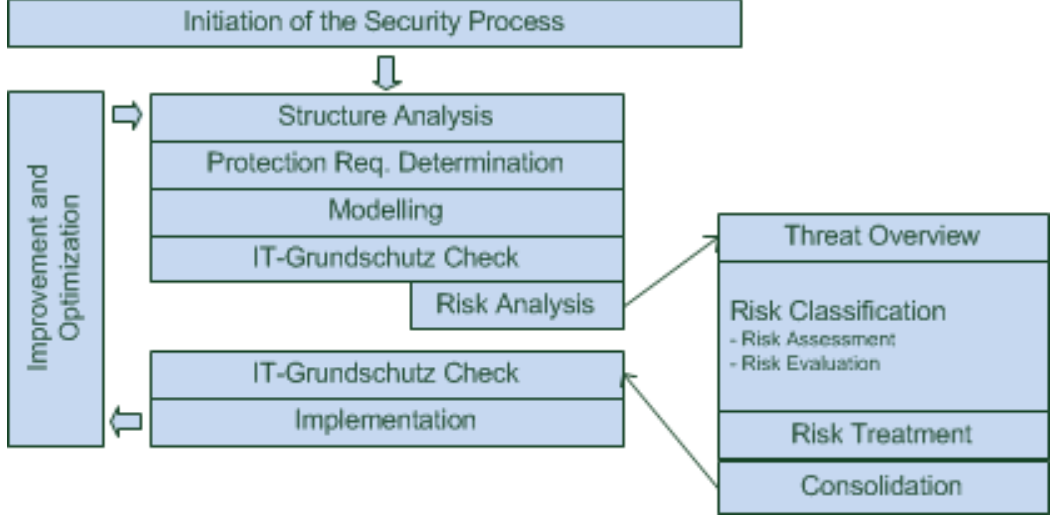
\includegraphics[width=\textwidth]{images/security-process-bsi-200-3.png}
  \textit{analýza rizík ako súčasť bezpečnostného procesu}
\end{frame}

\begin{frame}
  \frametitle{naša úloha}
  \begin{itemize}
    \item zákony 69/2018 Z. z. (ZoKB) a 95/2019 Z. z. (ZoITVS) ukladá povinnosť prevádzkovateľovi/správcovi
      vypracovať analýzu rizík
    \item nedostatok kvalifikovaných pracovníkov
    \item \textbf{úloha:} navrhnúť systém na podporu analýzy rizík pre malú organizáciu
  \end{itemize}
\end{frame}

\section{súčasný postup}
\begin{frame}
  \frametitle{súčasný postup}
  \begin{itemize}
    \item prešiel som si publikáciou o obciach, z ktorých vyplynulo niekoľko typických agend zahrňujúce IT systémy
  \end{itemize}
  \begin{center}
    
\includegraphics[height=15em]{images/prirucka-dobreho-starostu.png}
  \end{center}
\end{frame}
\begin{frame}
  \frametitle{súčasný postup}
  \begin{itemize}
    \item navrhol som jednoduchú pomôcku uľahčujúcu zaćiatok analýzy rizík
  \end{itemize}
  \begin{center}
    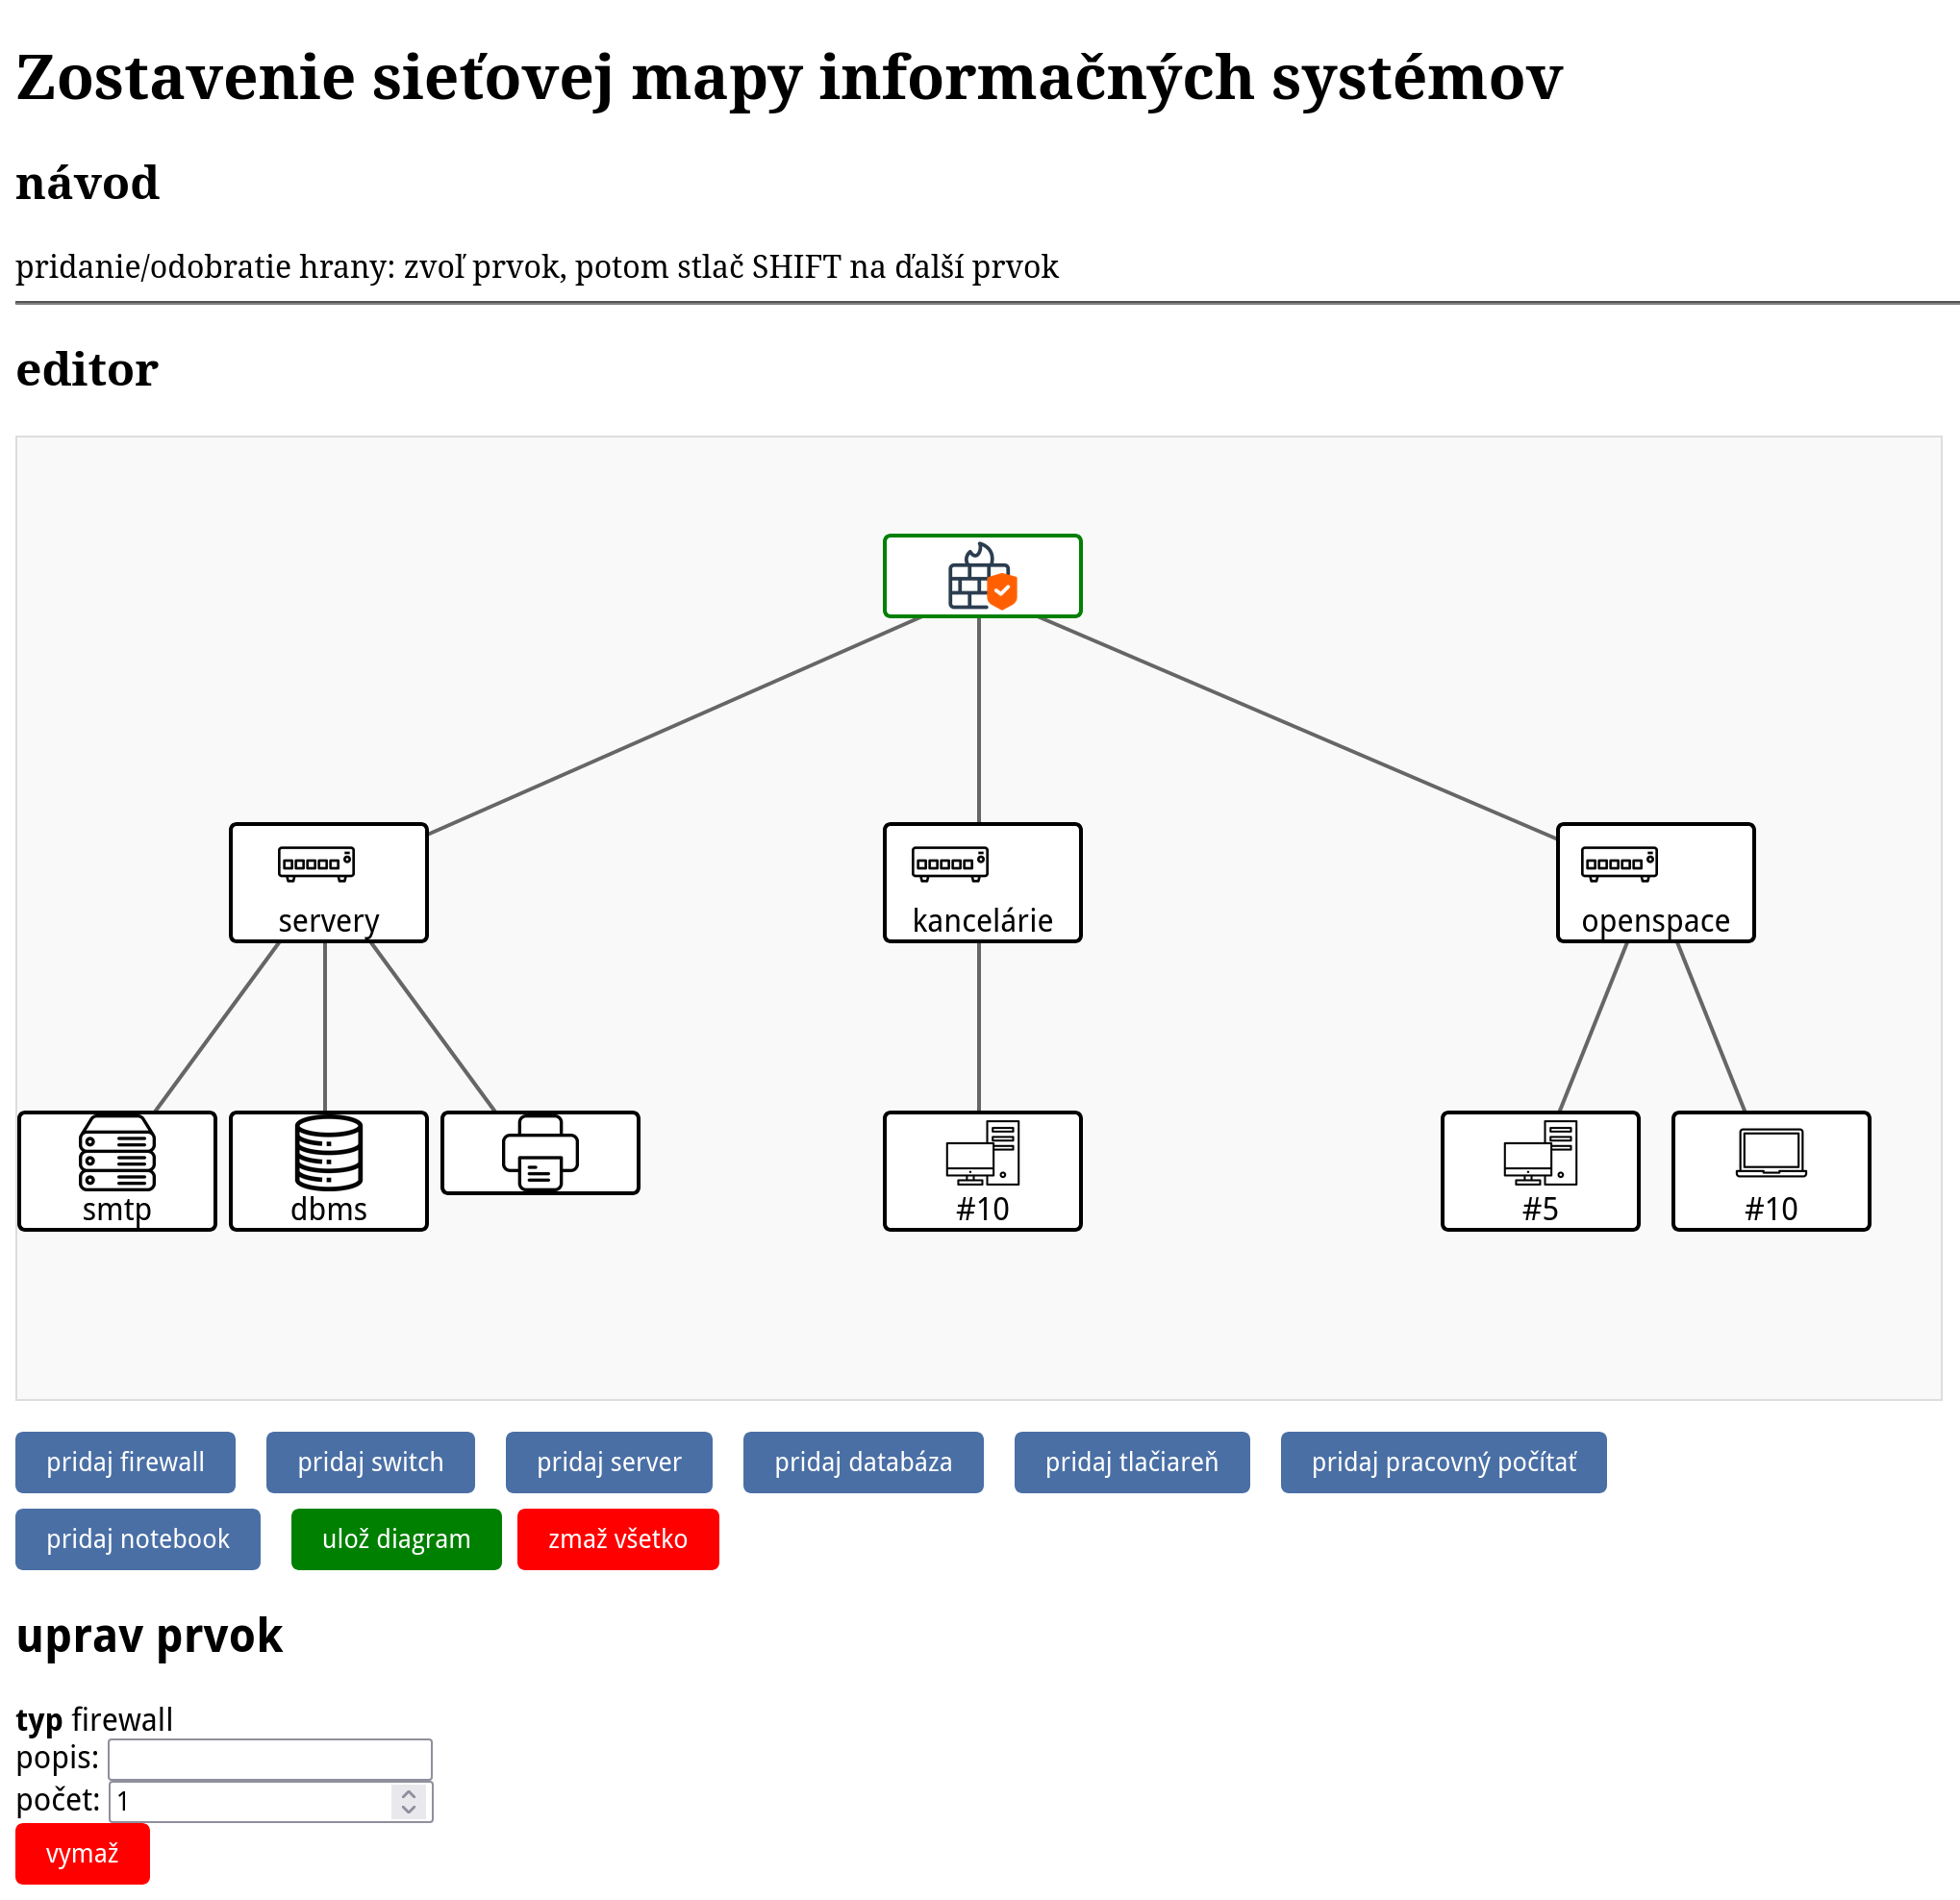
\includegraphics[height=15em]{images/it-network-map-visualizer.png}
  \end{center}
\end{frame}
\begin{frame}
  \frametitle{súčasný postup}
  \begin{itemize}
    \item preskúmal som susedné vzdelávanie Čechov v oblasti KIB
  \end{itemize}
  \begin{center}
    \includegraphics[width=\textwidth]{images/nukib.png}
  \end{center}
\end{frame}

\section{najbližšie v pláne}
\begin{frame}
  \frametitle{najbližšie v pláne}
  \begin{itemize}
    \item veľmi inštrumentálna pomôcka bola publikácia CyBOK
    \item preskúmať zdroje \textit{National Cyber Security Centre - NCSC.GOV.UK}
    \item preskúmať ďalšie publikácie pre metódy analýzy rizík ako:
      \begin{itemize}
        \item NIST SP-800-30 Risk Assessment Process
        \item Octave Allegro
        \item TOGAF - The Open Group Architecture Framework
      \end{itemize}
    \item preskúmať jazyk STIX (\textit{Structured Threat Information Expression)}
      a protokol TAXII™(\textit{Trusted Automated eXchange of Intelligence Information})
    \item pokračovať v prototypovaní funkcionality systému
  \end{itemize}
\end{frame}

\begin{frame}
  \frametitle{ďakujem za pozornosť}
\end{frame}
\end{document}
